\subsubsection{Каково различие между симметричным, асимметричным и резко асимметричным p-n переходами? В каких электронных приборах такие переходы встречаются?}

Прежде всего стоит заметить, что p-n переход нельзя осуществить путём простого соприкосновения двух разнородных пластинок, так как при этом неизбежен промежуточный (хотя бы и очень тонкий) слой воздуха или поверхностных плёнок. Настоящий переход получается в единой пластинке полупроводника, в которой тем или иным образом получена резкая граница между слоями p и n.

Резкость границы играет существенную роль для формирования перехода, так как чересчур плавный переход, как показывает теория, не обладает теми вентильными свойствами, которые лежат в основе работы полупроводниковых дидов и транзисторов. Понятие резкости формулируется следующим образом: граница между слоями является резкой, если градиент концентрации примеси(считающийся постоянным в пределах перехода) удовлетворяет неравенству:
\begin{equation}
\left|\frac{dN}{dx}\right|l_{Di} >> n_i
\label{condition}
\end{equation}

N - эффективная концентрация примеси(разность концентраций акцепторов и доноров), а $l_{Di}$ - дебаевская длина в собственном полупроводнике. (длина области, обогащенной носителями заряда)
Это неравество говорит о том, что концентрация примесей в переходе должна существенно изменяться на отрезке, меньшем $l_{Di}$. Такое требование имеет следующий физический смысл: если градиент $dN/dx$ очень мал, то существенные(сравнимые с $n_i$) эффективные концентрации получаются вдали от точки x=0,на расстояниях > $l_{Di}$. Тогда поля объемных зарядов, обусловленных ионизированными примесными атомами тоже будут расположены вдали от металлургической границы. Соответстветственно в окрестности металлургической границы не сможет образоваться двойной электрический слой, свойственный p-n переходу.
\pagebreak

Иллюстрация:
\begin{center}
	\begin{figure}[h!]
		\center{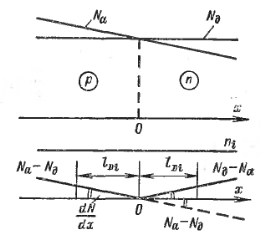
\includegraphics[scale=0.9]{N().png}}
		\caption{Распределение полных и эффективных концентраций примеси вблизи металлургической границы плавного перехода}
	\end{figure}
\end{center}

Переходы, в которых имеется скачкообразное изменение концентрации на границе слоев ($dN/dx = \inf$), называются \textbf{ступенчатыми}. Они представляют собой предельный слуай более общего класса \textbf{резких} переходов, в которых градиент концентрации примесей конечен, но удовлетворяет условию \ref{condition}. На практике ступенчатые переходы являются лишь приближением. Однако они хорошо отражают свойства многих реальных p-n структур и оказываются проще для анализа.

По соотношению концентраций основных носителей в слоях p и n переходы делятся на \textbf{симметричные} и \textbf{несимметричные}. В симметричных переходах имеет место соотношение 
$$
p_p \approx n_n
$$,
т.е. концентрации основных носителей в обоих слоях почти одинаковы. Такие переходы трудно реализовать практически и они не являются типичными. Гораздо большее распространение имеют несимметричные переходы, в которых выполняется неравенство:
$$
p_p > n_n \textit{ или } n_n > p_p
$$

и концентрации различаются в несколько раз и более. Именно такие переходы будут анализироваться в дальнейшем. В случае резкой асимметрии, когда концентрации основных носителей различаются более чем на порядок, переходы называют односторонними и обычно обозначают символами $p^+-n$ или $n^+-p$





